%! TEX program = lualatex
\documentclass[11pt]{scrartcl}
% Packages
\usepackage[margin=1.25in]{geometry}
\usepackage{index}
\usepackage{amsbsy} % Bold math symbols
\makeindex
\usepackage[utf8]{inputenc}
\usepackage[T1]{fontenc}
\usepackage{tcolorbox}
\tcbuselibrary{theorems}
\tcbuselibrary{skins}
\tcbuselibrary{breakable}
\usepackage{varwidth}
\usepackage{textcomp}
\usepackage{amsmath, amssymb}
\usepackage{esint}
\usepackage{titlesec}
\usepackage{xcolor}
\usepackage{titling}
\usepackage[linktocpage]{hyperref}
\usepackage{pgfplots}
\usepackage{multicol}
\setlength{\columnsep}{2em}
\usepackage{caption}
\usepackage{amsthm}
\usepackage{import}
\usepackage{cancel}
\usepackage{caption}
\usepackage{nicematrix}
\usepackage{mathrsfs}
\usepackage{mathtools}
%\usepackage{parskip}
\usepackage{pythonhighlight}
\usepackage{enumerate}
\usepackage{graphicx}
\usepackage{tikz}
\usepackage[italian]{babel}
\usepackage{setspace}
\setstretch{1.2}
% To reset footnote numbering each page
\usepackage[perpage]{footmisc}
\usepackage{faktor}

% Titles 
\title{Appunti di\\ \vspace{.3cm} Algebra}
\author{Manuel Deodato}
\date{}


\definecolor{mastercolor}{HTML}{5666a8}


\newtheoremstyle{style1}% name of the style to be used
{5pt}% measure of space to leave above the theorem. E.g.: 3pt
{5pt}% measure of space to leave below the theorem. E.g.: 3pt
{\normalfont}% name of font to use in the body of the theorem
{15pt}% measure of space to indent
{\sffamily\scshape\bfseries}% name of head font
{}% punctuation between head and body
{ }% space after theorem head; " " = normal interword space
{\thmname{#1}\thmnumber{ #2}{\thmnote{ (#3)}.\ }}

\theoremstyle{style1}
\newtheorem{osservazione}{Osservazione}[section]
\newtheorem{teorema}{Teorema}[section]
\newtheorem{prop}{Proposizione}[section]
\newtheorem{corollario}{Corollario}[teorema]
\newtheorem{lemma}{Lemma}[teorema]
\newtheorem{definizione}{Definizione}[section]
\newtheorem{notazione}{Notazione}[section]
\newtheorem{esempio}{Esempio}[section]
\newtheorem{esercizio}{Esercizio}[section]

\newenvironment{svolgimento}{\renewcommand\qedsymbol{$\blacksquare$}\begin{proof}[Svolgimento]}{\end{proof}}

%% Generic box
\newtcolorbox{eqbox}[1][]
{
colback=gray!10,
arc=0pt,
boxrule=0pt,
title=#1
}

 \newenvironment{boxenv}[1][]{
    \begin{eqbox}[#1]
    }{
   \end{eqbox}
}



%%%%%%%%%% Medie con integrali multipli
\def\Yint#1{\mathchoice
    {\YYint\displaystyle\textstyle{#1}}%
    {\YYint\textstyle\scriptstyle{#1}}%
    {\YYint\scriptstyle\scriptscriptstyle{#1}}%
    {\YYint\scriptscriptstyle\scriptscriptstyle{#1}}%
      \!\iint}
\def\YYint#1#2#3{{\setbox0=\hbox{$#1{#2#3}{\iint}$}
    \vcenter{\hbox{$#2#3$}}\kern-.51\wd0}}
\def\longdash{{-}\mkern-3.5mu{-}} 
   % consider using "\mkern-7.5mu" if esint package is loaded
\def\tiltlongdash{\rotatebox[origin=c]{15}{$\longdash$}}
\def\fiint{\Yint\tiltlongdash}

\def\Zint#1{\mathchoice
    {\YYint\displaystyle\textstyle{#1}}%
    {\YYint\textstyle\scriptstyle{#1}}%
    {\YYint\scriptstyle\scriptscriptstyle{#1}}%
    {\YYint\scriptscriptstyle\scriptscriptstyle{#1}}%
      \!\iiint}
      \def\tilongdash{\mkern6mu{-}\mkern-4mu{-}\mkern-5mu{-}} 
   % consider using "\mkern-7.5mu" if esint package is loaded
\def\titiltlongdash{\rotatebox[origin=c]{15}{$\tilongdash$}}
\def\fiiint{\Zint\titiltlongdash}

%Captions
\captionsetup[figure]{font=footnotesize,labelfont=footnotesize}
\captionsetup[table]{font=footnotesize,labelfont=footnotesize}
%Titlesec
\titleformat{\section}
{\fontsize{18}{20}\sffamily\scshape}
{\normalfont\color{mastercolor}{\fontsize{18}{20}\selectfont\thesection}}
{0.7em}
{}
\titlespacing*{\section}{0pt}{*2}{1cm}
\titlespacing*{\subsection}{0pt}{*5}{.5cm}
\titlespacing*{\subsubsection}{0pt}{*5}{.5cm}

\hypersetup{colorlinks,breaklinks, linkcolor=[RGB]{86, 102, 168}}

% Personalizza la formattazione della subsection
\titleformat{\subsection}[block]{\centering\fontsize{14}{20}\bfseries}{\normalfont\thesubsection}{.5em}{}


% Personalizza la formattazione della subsubsection
\titleformat{\subsubsection}[block]{\centering\fontsize{12}{20}\bfseries}{\normalfont\thesubsubsection}{.5em}{}

% Maketitle customization
\renewcommand{\maketitle}{
\begin{center}
{\sffamily
{\fontsize{20}{20}\selectfont\MakeUppercase\thetitle}}

\vspace{0.2in}

{\large\scshape\sffamily\theauthor}
\end{center}
}

%Evaluate symbol
\DeclareMathOperator{\di}{d\!}
\newcommand*\Eval[3]{\left.#1\right\rvert_{#2}^{#3}}

%%%%%%% Numero delle equazioni in formato a.b
\numberwithin{equation}{subsection}
%%%%%

%%%%%%%%%% Personalizzazione numeri lista
\renewcommand{\theenumi}{(\arabic{enumi})}

%%%% Table of contents

\usepackage[titles]{tocloft}

\renewcommand{\cftdot}{}
\usepackage{titletoc}
%\setcounter{tocdepth}{2}

%%%%%%%%%%%%%%%% Toc style

% Personalizzazione scritta indice


% Font
\usepackage{helvet}
\renewcommand{\familydefault}{\sfdefault}	
\renewcommand{\operatorname}[1]{\mathop{\mathrm{\textsf{#1}}}}
\usepackage[noSTIXops,scaled=1.1]{newtxsf}


\begin{document}
\maketitle
\vspace{9cm}
\begin{figure}[h!]
	\centering
	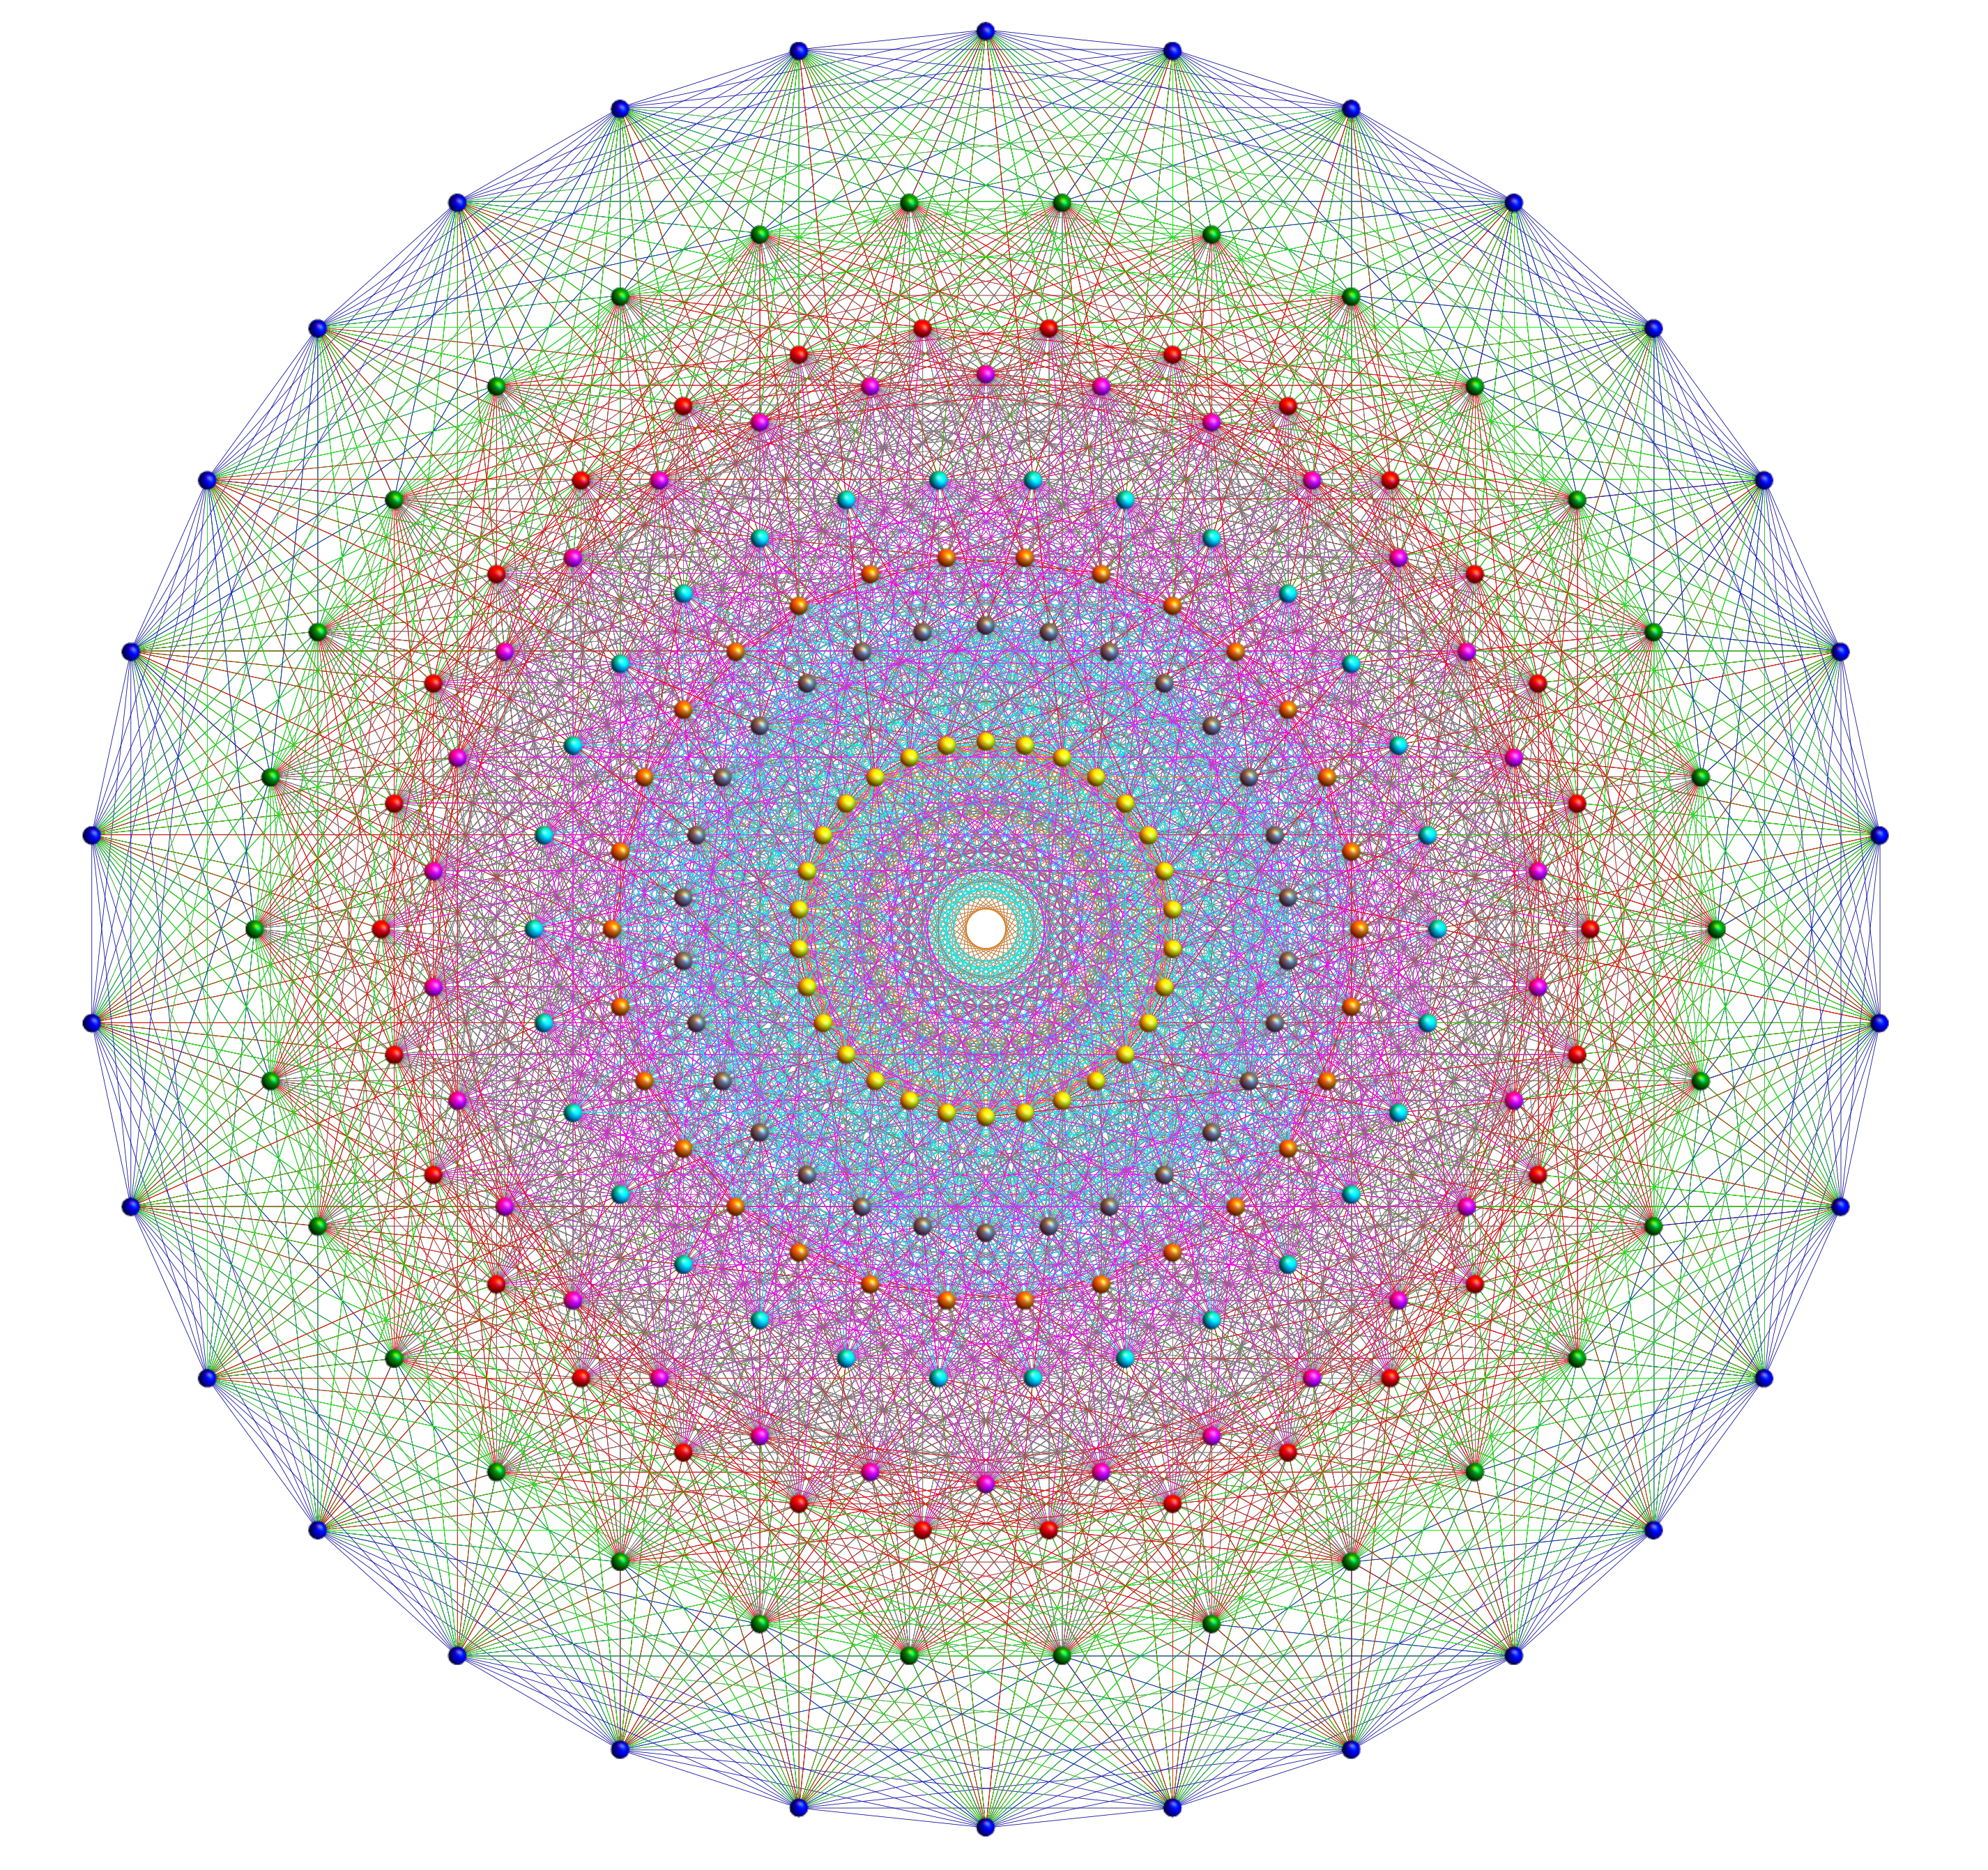
\includegraphics[width=.8\columnwidth]{front.jpeg}
\end{figure}

\newpage
\tableofcontents 
\newpage
\section{Teoria dei gruppi}
\subsection{Il gruppo degli automorfismi}
\begin{lemma}
	Siano $H,G$ due gruppi ciclici; un omomorfismo $\varphi : G \to H$ \`e univocamente determinato da come agisce su un generatore di $G$.
	\begin{proof}
		Sia $g_0\in G$ tale che $\langle g_0 \rangle = G$ e sia $\varphi (g_0) = \overline{h}\in H$.
		Per $g \in G$ generico, per cui $g_0^k = g$ per qualche intero $k$, si ha:
		\[
		\varphi (g) = \varphi (g_0^k) = \varphi (g_0)^k = \overline{h}^k
		\] 
		Cio\`e tutti gli elementi di $\operatorname{Im} \varphi $ sono esprimibili come potenze di $\overline{h}$.
	\end{proof}
\end{lemma}
\begin{osservazione}
Non ogni scelta di $\overline{h} \in H$ \`e ammissibile, ma bisogna rispettare l'ordine di $g_0$.
Se $g_0^n = e_G$, allora $e_H = \varphi (g_0^n) = \varphi (g_0)^n = \overline{h}^n$. Questa condizione, impone che $\operatorname{ord}(\overline{h})  \mid \operatorname{ord}(g_0) $.
\end{osservazione}
\begin{definizione}
	[Gruppo degli automorfismi]
	Sia $G$ un gruppo; si definisce il gruppo dei suoi automorfismi come
	\[
	\operatorname{Aut} (G) = \left\{ f: G \to G  \mid f \text{ \`e un isomorfismo di gruppi} \right\} 
	\] 
\end{definizione}
\begin{esempio}
	Si calcola $\operatorname{Aut} (\mathbb{Z})$. 
	\begin{svolgimento}
		Il gruppo $(\mathbb{Z},+)$ \`e ciclico, quindi un omomorfismo \`e determinato in base a come agisce su un generatore.
		Prendendo, per esempio $1$, si definisce $q_a :\mathbb{Z}\to \mathbb{Z} $ tale che $ q_a (1 ) = a$; perch\'e $\langle q_a(1) \rangle = \mathbb{Z}$\footnote{Richiesto dal fatto che $q_a$ sia suriettivo.}, \`e necessario che $a$ sia un generatore di $\mathbb{Z}$, perci\`o sono ammessi $a = \pm 1$. 
		In questo caso, $\operatorname{Aut} (\mathbb{Z})=\left\{ \pm \operatorname{Id} _{\mathbb{Z}}  \right\} \cong \left(\mathbb{Z} / 2\mathbb{Z}, +\right) $.
	\end{svolgimento}
\end{esempio}
\begin{teorema}
$\operatorname{Aut} (\mathbb{Z} / m \mathbb{Z}) \cong (\mathbb{Z} / m \mathbb{Z})^*$.
\begin{proof}
	$(\mathbb{Z} / m\mathbb{Z}, + )$ \`e ciclico, quindi si stabilisce l'azione di $f:\mathbb{Z} / m\mathbb{Z}\to \mathbb{Z}/ m\mathbb{Z}$ su un generatore.
	Preso, allora, $\overline{k} \in \mathbb{Z} / m\mathbb{Z} $ tale che $\operatorname{gcd}(k,m) =1$ e scelto $f(\overline{k}) = \overline{a}$, si ha che $\langle f(\overline{k}) \rangle= \langle \overline{a} \rangle= \mathbb{Z} / m\mathbb{Z} \iff \operatorname{gcd}(a,m) =1	\iff \overline{a} \in \left(\mathbb{Z} / m\mathbb{Z}\right) ^* $.
\end{proof}
\end{teorema}
\begin{definizione}
	[Automorfismo interno]
	Sia $G$ un gruppo; si definisce $\phi _g :G\to G$, $ \forall g \in G$, come $\phi_g (x) =gxg^{-1} $ ed \`e detto \textit{automorfismo interno}. 
	L'insieme di questi automorfismi, al variare di $g \in G$, forma il gruppo
	\[
	\operatorname{Int} (G) = \left\{ \phi _g : G\to G  \mid g \in G \text{ e } \phi _g \text{ automorfismo interno} \right\} 
	\] 
\end{definizione}
\begin{prop}\label{intcar}
	Sia $G$ un gruppo; allora $\operatorname{Int} (G) \lhd \operatorname{Aut} (G)$ e $\operatorname{Int} (G) \cong G / Z(G)$.
	\begin{proof}
		$\operatorname{Int} (G)$ \`e un sottogruppo di $\operatorname{Aut} (G)$ perch\'e $\operatorname{Id} (x) = exe^{-1} = x  \Rightarrow \operatorname{Id} \in \operatorname{Int} (G)$.
		Inoltre, $\phi _g \circ \phi _h (x) = ghxh^{-1}g^{-1}=\phi _{gh} (x) \in \operatorname{Int} (G)$ e $\phi _{g^{-1} } \circ \phi _g (x) = x \Rightarrow \phi _g^{-1} = \phi _{g^{-1}} \in \operatorname{Int}(G)  $.

		\`E un sottogruppo normale perch\'e $\forall f \in \operatorname{Aut} (G)$, si ha 
		\[
		f \circ \phi _g \circ f^{-1}(x) = f \left(g f^{-1}(x) g^{-1}\right) =f(g) x f(g)^{-1} \in \operatorname{Int} (G)
		\] 
		Per finire, si definisce $\Phi : G \to \operatorname{Int} (G) $.
		Questo \`e un omomorfismo perch\'e $\Phi(gh)=\phi _{gh} = \phi _g\circ \phi _h = \Phi(g)\Phi(h)$.
		\`E, inoltre, suriettivo perch\'e ogni automorfismo interno \`e associato ad un elemento di $G$, cio\`e $\forall \phi _g \in \operatorname{Int} (G), \ \exists g \in G : \Phi(g) = \phi _g$.
		Allora, la tesi deriva dal I teorema di omomorfismo, visto che $\operatorname{Ker} \Phi = Z(G)$.
	\end{proof}
\end{prop}
\begin{osservazione}\label{ossnorm}
	$H \lhd G \iff \phi _g(H) = H, \ \forall \phi _g \in \operatorname{Int} (G)$.
	\begin{proof}
Per ogni elemento di $\operatorname{Int} (G)$, si ha $\phi _g (H) = H \iff gH g^{-1} = H \iff H \lhd G$.
	\end{proof}
	\end{osservazione}
\begin{definizione}
	[Sottogruppo caratteristico]
	Sia $G$ un gruppo e $H < G$. Si dice che $H$ \`e \textit{caratteristico} se \`e invariante per automorfismo, cio\`e $\forall f \in \operatorname{Aut} (G), \ f(H) = H$.
\end{definizione}
\begin{corollario}
	Sia $G$ un gruppo; per la proposizione \ref{intcar} e l'osservazione \ref{ossnorm} se $H$ \`e caratteristico, allora $H \lhd G$.
\end{corollario}
\noindent Il viceversa \`e falso, cio\`e normale $\not\Rightarrow $ caratteristico; infatti, in $\mathbb{Z} / 2\mathbb{Z} \times  \mathbb{Z} / 2\mathbb{Z}$, il sottogruppo $\langle (1,0) \rangle$ \`e normale, ma non caratteristico perch\'e l'automorfismo che scambia le coordinate \`e tale per cui $\langle (1,0) \rangle\mapsto \langle (0,1) \rangle\neq \langle (1,0) \rangle$.
\subsection{Azioni di gruppo}
\begin{definizione}
	[Azione]
	Sia $G$ un gruppo; un'azione di $G$ su un insieme $X$ \`e un omomorfismo
	\[
	\gamma : 
	\begin{array}
		{c c c}
		G &\longrightarrow & S(X) = \left\{ f : X \to X  \mid f \text{ biettiva} \right\} \\
		g & \longmapsto & \psi _g : \psi_g(x) = g \cdot x
	\end{array}
	\] 
\end{definizione}
\begin{esempio}
Sia $G = \left\{ z \in \mathbb{C}^*  \mid  \lvert z \rvert =1 \right\} \cong S^1$ la circonferenza unitaria e $X = \mathbb{R}^2$.
Un'azione di $G$ su $X$ \`e una rotazione definita da $\gamma(z) = R(\operatorname{arg} z)$.
Questa \`e un omomorfismo perch\'e $\gamma(zw) = R(\operatorname{arg} zw)  = R(\operatorname{arg} z +  \operatorname{arg} w) = R(\operatorname{arg} z) R(\operatorname{arg} w)= \gamma(z) \gamma(w)$.
\end{esempio}
\noindent Un'azione $\gamma$ di $G$ su $X$ definisce, proprio su $X$, una relazione di equivalenza definita da 
\begin{equation}
	x \sim _\gamma y \iff x=\psi _g(y)=g \cdot y, \text{ con } x,y \in X
\end{equation}
La relazione di equivalenza \`e ben definita perch\'e le $\psi _g$ sono mappe biettive.
\begin{definizione}
	[Orbita]
	Sia $\gamma :G \to S(X)$ un'azione di $G$ gruppo su $X$. Dato $x \in X$, la sua classe di equivalenza rispetto alla relazione $\sim _\gamma$ \`e detta \textit{orbita} ed \`e indicata con $\operatorname{orb} (x) = \left\{ g \cdot  x  \mid g \in G\right\} $.
\end{definizione}
\noindent Ricordando che una relazione di equivalenza fornisce una partizione dell'insieme su cui \`e definita, si ha:
\begin{equation}
	X = \bigsqcup_{x \in R} \operatorname{orb} (x)
\end{equation}
con $R$ insieme dei rappresentati di tutte le orbite.
Se, poi, $X$ ha cardinalit\`a finita, allora:
\begin{boxenv}[]
\begin{equation}
	\lvert X \rvert  = \sum_{x \in R}^{} \lvert \operatorname{orb} (x) \rvert 
\end{equation}
\end{boxenv}
\begin{definizione}
	[Stabilizzatore]
	Sia $\gamma: G \to S(X)$ un'azione di $G$ su $X$; allora per ogni $x \in X$, si definisce l'insieme 
	\[
	\operatorname{Stab} (x) = \left\{ g \in G  \mid g \cdot  x = x \right\} < G 
	\] 	
\end{definizione}
\begin{lemma}\label{l111}
Se due elementi di un'orbita sono uguali, allora appartengono alla stessa classe di equivalenza di $G / \operatorname{Stab} (x)$.
\begin{proof}
	Se $g \cdot x, \ h\cdot x \in \operatorname{orb} (x)$ sono uguali, allora $x =h^{-1} g \cdot x $, cio\`e $h^{-1} g \in G$ lascia invariato $x$, quindi \`e in $\operatorname{Stab} (x)$.
	Da questo segue che $h \operatorname{Stab} (x) = h h^{-1} g \operatorname{Stab} (x) = g \operatorname{Stab} (x)$.
\end{proof}
\end{lemma}
\begin{prop}
	Esiste una mappa biettiva $\Gamma : \operatorname{orb} (x) \to G / \operatorname{Stab} (x)$ tale che $\Gamma(g \cdot x) = g \operatorname{Stab} (x)$.
	\begin{proof}
		$\Gamma$ \`e iniettiva come diretta conseguenza del lemma \ref{l111} ed \`e suriettiva perch\'e $\forall g \operatorname{Stab} (x) \in G / \operatorname{Stab} (x), \exists g\cdot x \in \operatorname{orb} (x)$ tale che $\Gamma(g\cdot x) = g \operatorname{Stab} (x)$.
	\end{proof}
\end{prop}
\end{document}
